\documentclass{article}
\usepackage{amsmath, graphicx, amsfonts, caption, subfig, keyval, algorithm, algorithmic}
\captionsetup{justification=centering}
\newcommand{\R}{\mathbb{R}}
\newcommand{\C}{\mathcal{C}}
\newcommand{\X}{\mathcal{X}}
\DeclareMathOperator*{\argmin}{\arg\!\min}

\begin{document}
\title{Weighted $k$-Centers \& Lloyd's Algorithm}
\author{Jonathan Friedman \& Taylor Killian}
\maketitle

\begin{abstract}
When determining the optimal location of distribution centers (e.g. warehouses, regional retail, or neighborhood commercial property), consideration must be made to maximize customer utility. It is assumed that individuals prefer the distance from them to any distribution center be minimized. To select the optimal location of distribution centers that minimize the average person's distance from any center, Lloyd's algorithm was altered to solve a variant of weighted $k$-centers. This augmented clustering algorithm was used to simulate a variety of distribution paradigms (differentiated by the weighting function used) using the 2010 U.S. Census population data for Massachusetts which provides a dense decision surface to optimize over. Results reaffirm the intuition that dense areas of high population are optimal locations to place centers. These solutions are highly dependent on the granularity of the data and how the population at each data point is weighted. 

\end{abstract}

\section{Introduction} \label{introduction}
Serving the maximum number of people at minimum expense is an important, canonical problem in industry. A company must balance placing their distribution centers near as many people as possible with the cost associated with opening and maintaining a large number of centers. A general formulation of this problem known as the metric $k$-center problem asks for a placement of $n$ distribution centers that minimizes the maximum distance from any point to a center \cite{kmeans}. In this paper, we examine the variant in which each point has a weight that affects its distance from the center point; in this case, the weight is a function of the population at the point. We also seek to minimize the sum of the maximum distances rather than the maximum individual distance. Efficient algorithms to solve this problem exist in one dimension \cite{1D}. For the two-dimensional case, we adapt Lloyd's algorithm, a clustering algorithm commonly applied to this type of problem, to work on this space by modifying the clustering step. 

If no attempt is made to avoid local extrema, then this problem is easy to solve for one center. In section \ref{onecenter}, we give a solution for one center using compass search. However, compass search is not viable for a large number of points because the number of required directions to search grows quickly. In section \ref{multicenters}, we give a solution method for an arbitrary number of centers using the modified Lloyd's algorithm. In section \ref{experiments}, we use our algorithm to optimize placement of distribution centers in Massachusetts based on population data from the U.S. 2010 Census, as well as to find the minimum number of distribution centers that produces a solution with a cost function below a specified tolerance level.

\section{Background \& Data} \label{background}
\subsection{Background}
Let $\C$ be the set of distribution centers, let $\X$ be the set of points which the centers serve, and let $d$ be a distance metric. In the general metric $k$-center problem, the goal is to minimize

$$\max_{p_i \in \X} \min_{c \in \C} d(c, p_i)$$

Now let $\xi_i$ be the population at point $p_i \in \X$, and $w$ be a weight function (we consider only weight functions where $\xi_i > \xi_j \implies w(\xi_i) \geq w(\xi_j)$, but more exotic weighting functions could be useful in other contexts). In the version of the weighted $k$-center problem that we consider, the goal is to minimize our cost function, the ``weighted mean distance" function

$$\frac{\sum_i w(\xi_i) \min_{c \in \C} d(c, p_i)}{|\X|}$$

Note that while the minimum achieved in the standard metric $k$-center problem corresponds to distance, the minimum achieved in the weighted problem does not have a direct physical interpretation. When $w$ is the identity function, it corresponds to minimizing the distance from the average person, rather than the average point, to its nearest distribution center. In general, it can be intuitively thought of as a weighted analogue to this mean distance, but its precise interpretation depends on the domain and context of the problem.

The choice of $w$ is also context and domain dependent. 
%check if this pans out
A superlinear $w$ could be used in a situation in which it is not as useful to place distribution centers near areas of low population density; for example, an expensive specialty store might place great importance on serving urban areas. A sublinear $w$ could be used in a situation in which optimally serving areas of high population density is not important, as in the case of a big-box retailer that customers generally visit infrequently.

Unless otherwise specified, $d$ is the standard Euclidean distance. Of course, this distance metric does not capture the true surface distance between points on the Earth. Since we test our algorithm on geographic data, we should, strictly speaking, use a different distance function such as the haversine formula; however, Euclidean distance provides a good approximation on small regions such as the state of Massachusetts. This region is small enough that the curvature of the Earth is effectively negligible when calculating the distance between two points.

\subsection{Census Data}
Throughout the paper, we test our algorithms using census block population data for Massachusetts from the 2010 U.S. Census. A census block is the smallest geographic unit for which population data is collected for every resident. Population data on a block level is available at \cite{census}, and can be parsed using geographic information software such as the Python Shapefile Library \cite{pyshp}. To generate a representative point for each block, we enclose the block in a bounding rectangle, then take the center of that rectangle to be the location of the block.

Although the 2010 Census divided Massachusetts into 157,508 total census blocks, 61,174 of those blocks have a population of zero (since every point in the United States is within a census block, and since census blocks are often delimited by geographical features, many blocks are partially or totally located in lakes, national parks, shopping malls, and so forth) \cite{blocks}. We ignore these blocks in our analysis because they are of little interest in the context of placing distribution centers to serve potential customers.

\section{One Distribution Center} \label{onecenter}
When $k=1$, the weighted $k$-centers problem is easily solved via compass search. Compass search is a simple method of minimizing a function $f : \R^n \rightarrow \R$ that does not require computation of the gradient. The algorithm is described in Algorithm \ref{alg:compass} (see \cite{survey} for further details).

\begin{algorithm}
  \caption{Compass Sort}
  \label{alg:compass}
\begin{algorithmic}
  \STATE  Let $\lambda_1,...,\lambda_m$ be a positive spanning set of $\R^n$. Choose a starting guess $p_0$, a step size $s_0$, a scaling constant $\alpha<1$, and a tolerance $t$.
  \WHILE{$s_k > t$}
  \IF{$f(p_k + s_k\lambda_i) < f(p_k)$ for some $\lambda_i$}
  \STATE $p_{k+1} = p_k + s_k\lambda_i$
  \STATE $s_{k+1} = s_k$
  \ELSE
  \STATE $p_{k+1} = p_{k}$
  \STATE $s_{k+1} = \alpha s_k$
  \ENDIF
  \ENDWHILE
  \RETURN $p_{k+1}$
\end{algorithmic}
\end{algorithm}

As above, we choose $f$ to be

$$\frac{\sum_i w(\xi_i) d(c, p_i)}{|\X|}$$.

Figure \ref{fig:popscale} shows distribution center placement for various $w$. As expected, the distribution center is consistently placed near Boston. Under $w(x) = \sqrt{x}$, the center moves farther away from Boston as the influence of high population to the objective function is decreased, and under $w(x) = x^2$, the center moves closer to Boston. However, the choice of weighting function appears to have little effect on placement of the center. Even when population is not taken into account, the center remains fairly close to Boston by virtue of the large number of census blocks located there.

\begin{figure}[!ht]%
  \centering
  \subfloat[$w(\alpha_i)=\alpha_i$]{{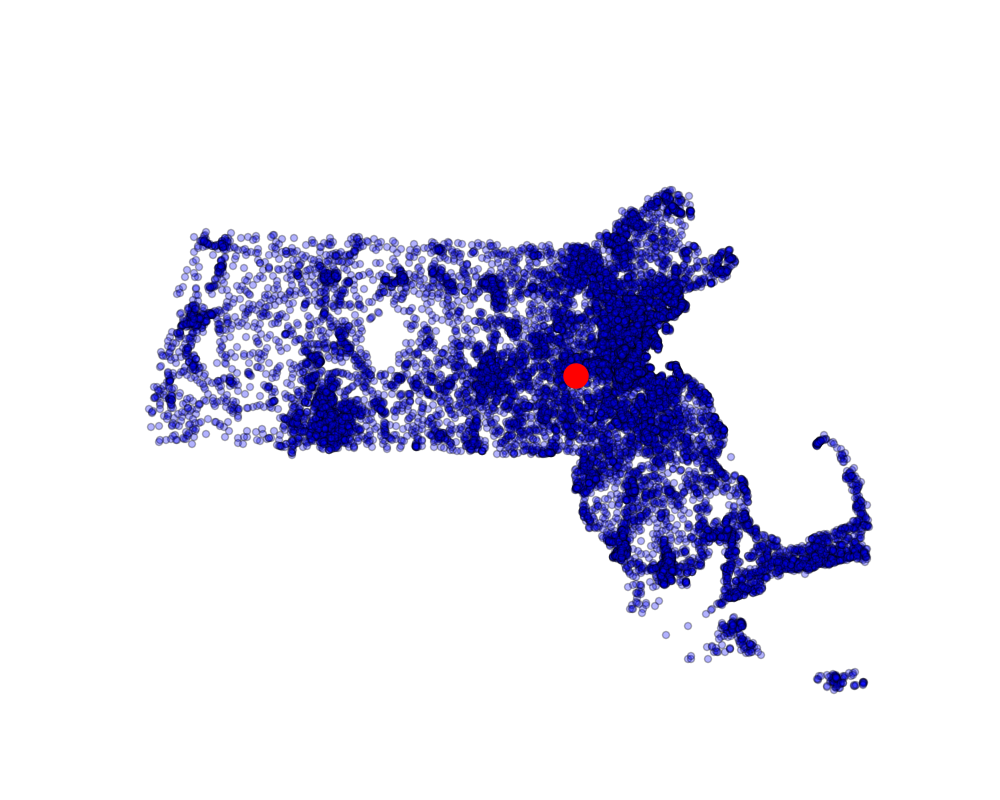
\includegraphics[width=5.5cm]{images/linweight.png} }}%
  \qquad
  \subfloat[$w(\alpha_i)=\sqrt{\alpha_i}$]{{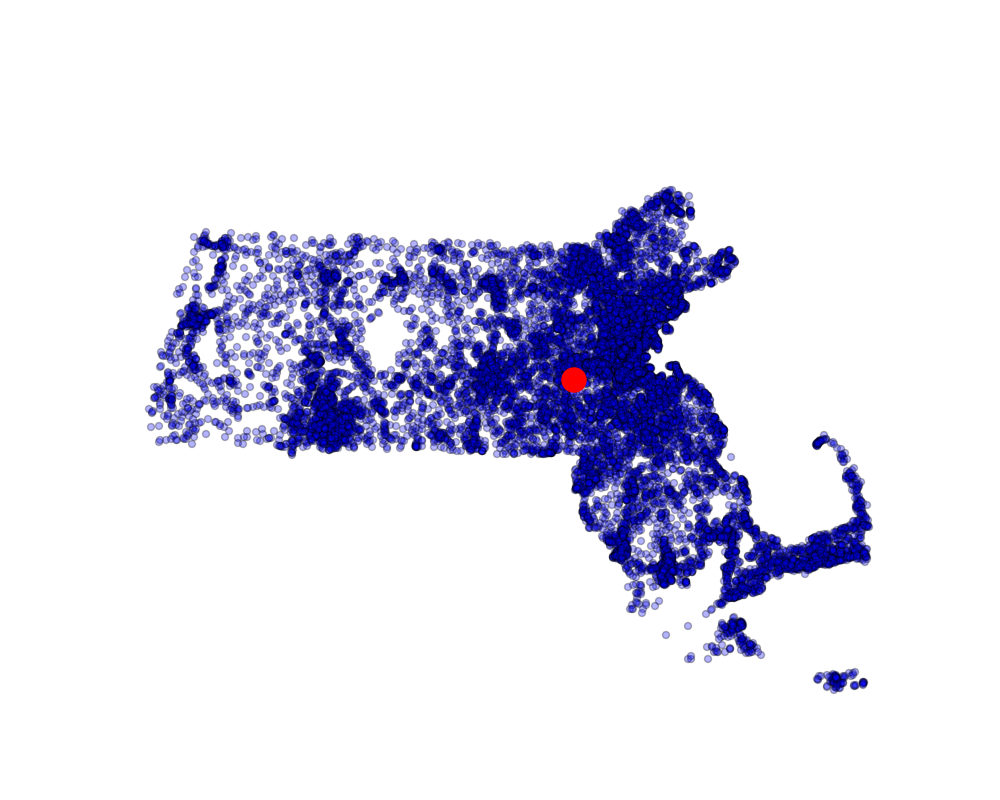
\includegraphics[width=5.5cm]{images/sqrtweight.png} }}%
  \qquad
  \subfloat[$w(\alpha_i)=\alpha_i^2$]{{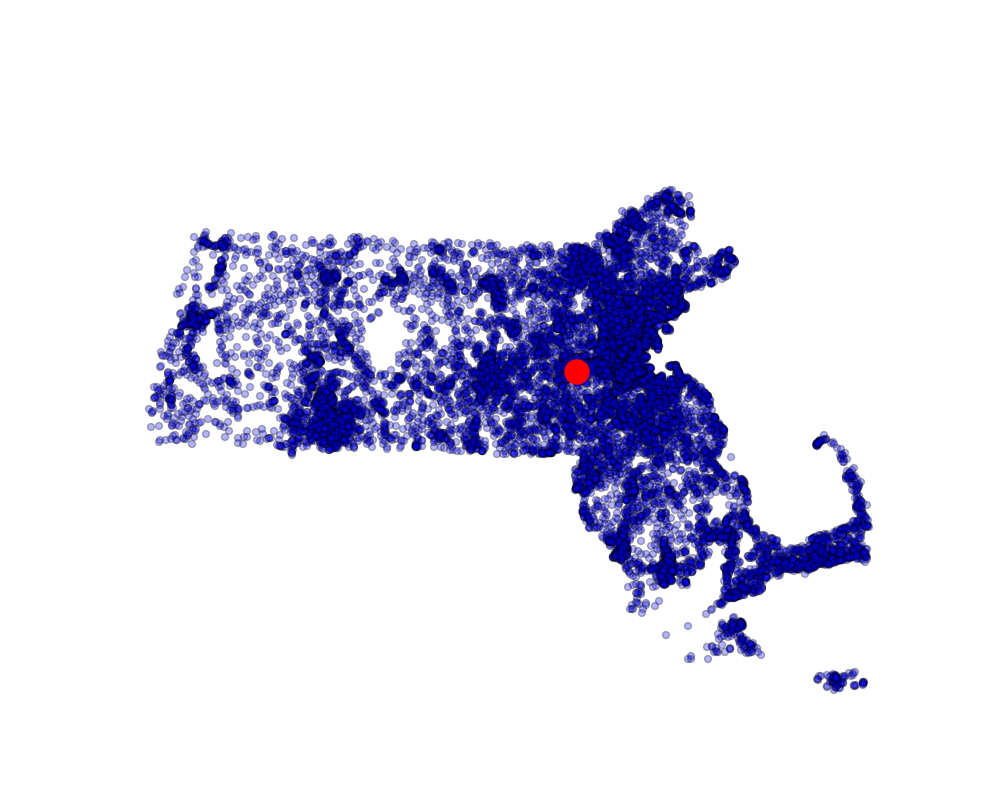
\includegraphics[width=5.5cm]{images/sqweight.png} }}%
  \qquad
  \subfloat[$w(\alpha_i)=1$]{{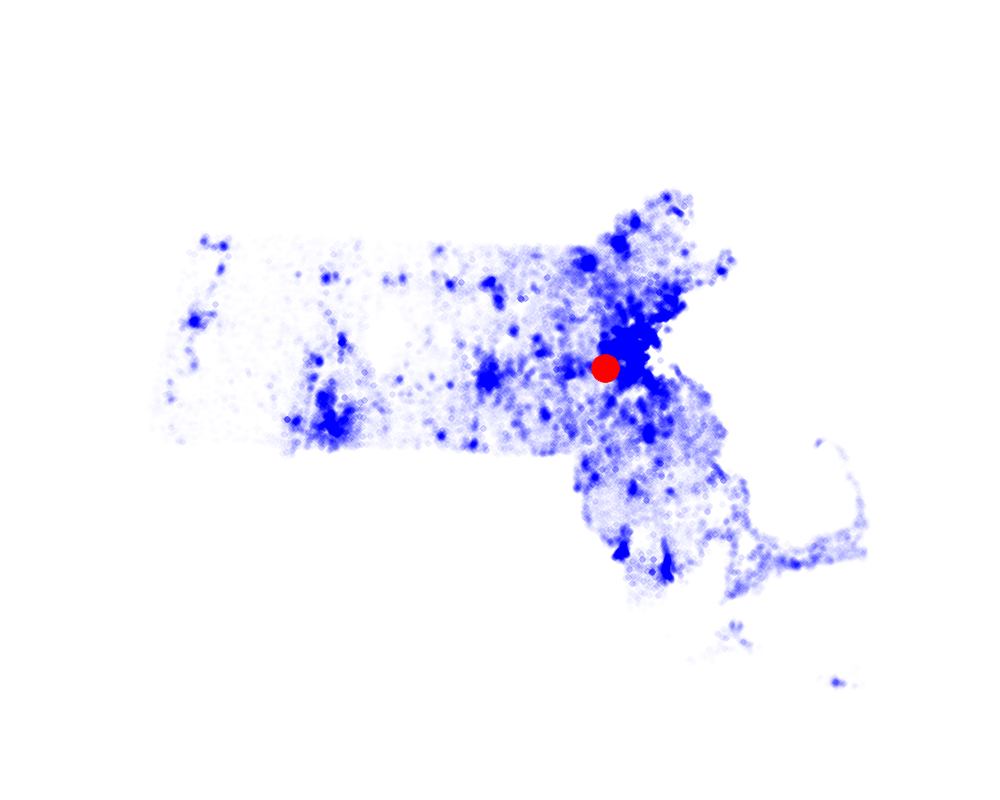
\includegraphics[width=5.5cm]{images/noweight.png} }}%
  \qquad
  \subfloat[][$w(\alpha_i)=\begin{cases}\alpha_i, & \alpha_i > 1\\ 0, & \text{otherwise} \end{cases}$]{{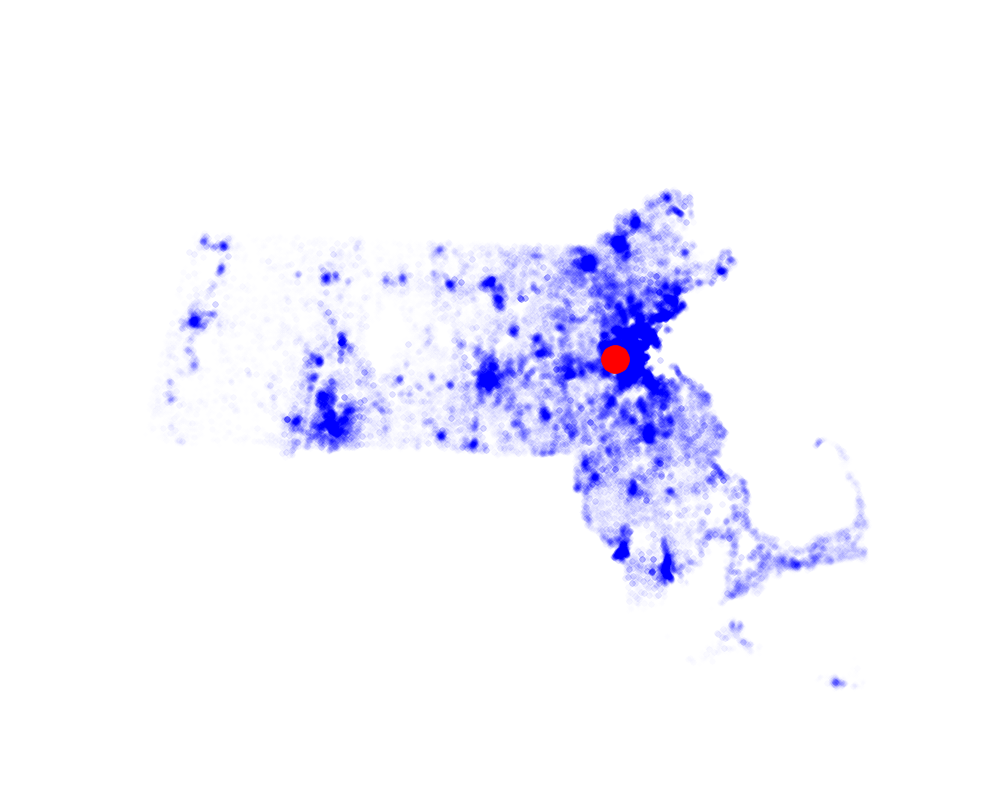
\includegraphics[width=5.5cm]{images/thresholdweight.png} }}
  \caption{Distribution center placement under various weighting \\ functions. The centers are shown in red.}
  \label{fig:popscale}
\end{figure}

This method works well for one distribution center, but the number of directions to search grows quickly with the number of centers.  Consider the case of $n$ clusters $c_1, ..., c_n \in \R^2$. Our function to minimize is now the full weighted mean distance function

$$\frac{\sum_i w(\xi_i) \min_{c \in \C} d(p_i, c)}{|\X|}$$

A positive spanning set for $\R^n$ must contain at least $n+1$ vectors \cite{charles}, so we must consider up to three possible directions at each step for each $p_i$. Determining the exact number of directions that must be searched for $n$ points in order to guarantee convergence to some maximum is beyond the scope of this report. Suffice it to say that better, more scaleable methods exist.

\section{Multiple Distribution Centers} \label{multicenters}
Lloyd's algorithm provides a more scaleable solution for multiple distribution centers. This algorithm was originally applied to problems in information theory \cite{lloyd}, but has been adapted to other fields such as clustering. A detailed description is given in Algorithm \ref{alg:lloyd} (see \cite{kmeans} for further details).The general algorithm works as follows: first, assign, via some method, starting locations for the centers. Then, assign each center a cluster $\Gamma$ composed of points closer to it than to any other center. Next, iteratively move the centers to the centers of their respective Voronoi cells. Repeat until the centers do not move between iterations. Therefore in the center adjusting step, rather than relocating the center to the geographical mean, we find the new location for a center $c$ in cluster $\Gamma$ by solving the optimization problem

$$\argmin_{c} \sum_{\{i: p_i \in \Gamma\}} w(\xi_i) d(p_i, c)$$

This is equivalent to finding a root of the gradient

$$\Bigg[ \sum_{\{i: p_i \in \Gamma\}} w(\xi_i) \Big(\frac{p_{ix} - c_x}{d(p_i, c)}\Big), \sum_{\{i: p_i \in \Gamma\}} w(\xi_i) \Big(\frac{p_{ix} - c_y}{d(p_i, c)}\Big) \Bigg]^T$$

We randomly assign starting centers, though other initialization methods may be used. This suffices to find a solution for an arbitrary number of distribution centers.

\begin{algorithm}
  \caption{Lloyd's Algorithm with Weighting}
  \label{alg:lloyd}
\begin{algorithmic}
  \STATE  Randomly choose $n$ initial centers $\{c_1^1, ..., c_n^1\}=\C$, and let $\{\gamma_1, ..., \gamma_n\}=\Gamma$ be their corresponding clusters. 
  \WHILE {$\exists c_i : c_i^k \neq c_i^{k-1}$}
  \FOR{$\gamma_i \in \Gamma$}
    \STATE $\gamma_i = \{x \in \X : d(x, c_i^k) < d(x, c_j^k) \ \forall j \neq i\}$
  \ENDFOR
  \FOR{$c_i \in \C$}
    \STATE $c_i^k = \argmin_{\chi} \sum_{\{i : p_i \in \gamma\}} w(\xi_i) d(p_i, \chi)$
  \ENDFOR
  \ENDWHILE
\end{algorithmic}
\end{algorithm}

To find a solution such that the cost function is below a given threshold and the number of centers is minimized, run the algorithm for $1, 2, ...$ centers until the cost function falls below the threshold. Lloyd's algorithm is not guaranteed to produce a global minimum, so to more fully explore the space, we run the algorithm several times, stochastically varying the initialization points, for each choice of $k$.

\section{Experiments} \label{experiments}
As in the case of one distribution center, we test our algorithm on U.S. census data from Massachusetts. In order to compare results with the same tolerance and different $w$, we develop a simple rescaling such that under each $w$, all calculated weights satisfy $\{w(\xi_i) \in [0,1] \ \big| \ \sum_i w(\xi_i) = 1\}$. Initially, we solve the problem of placing the minimum number of centers such that the weighted mean distance with $w(\xi) = \xi$ is below a given initial tolerance level. Then, for every other weighting function $w$, we solve the problem for under that same tolerance.

\subsection{Rescaling} \label{rescaling}
Without rescaling, it is difficult to compare results with different choices of $w$. For example, the weighted mean distance with $w(\xi) = \xi^2$ will necessarily be much greater than the weighted mean distance with $w(\xi) = \sqrt{\xi}$. Therefore, we divide both the tolerance and the cost function by

$$\sum_i w(\xi_i)$$

This roughly corresponds to a rescaling to the same scale of the case when $w(\xi) = \xi$. Rescaling the tolerance is equivalent to choosing a smaller tolerance to start with. However, rescaling is a systematic way of converting a tolerance with a physical interpretation to one suited to the problem. 

\subsection{Minimum Distribution Centers}
Figure \ref{fig:centers} shows the results of generating 10 clusters under five different weighting functions. 
\begin{figure}[!ht]%
  \centering
  \subfloat[$w(\xi)=\xi$]{{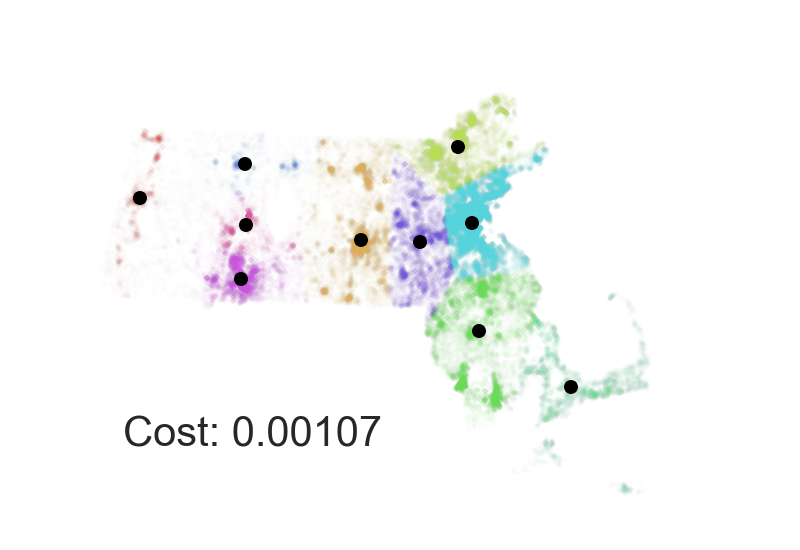
\includegraphics[width=5.5cm]{images/solution_linwt_clusters10_minpop1.png} }}%
  \qquad
  \subfloat[$w(\xi)=\sqrt{\xi}$]{{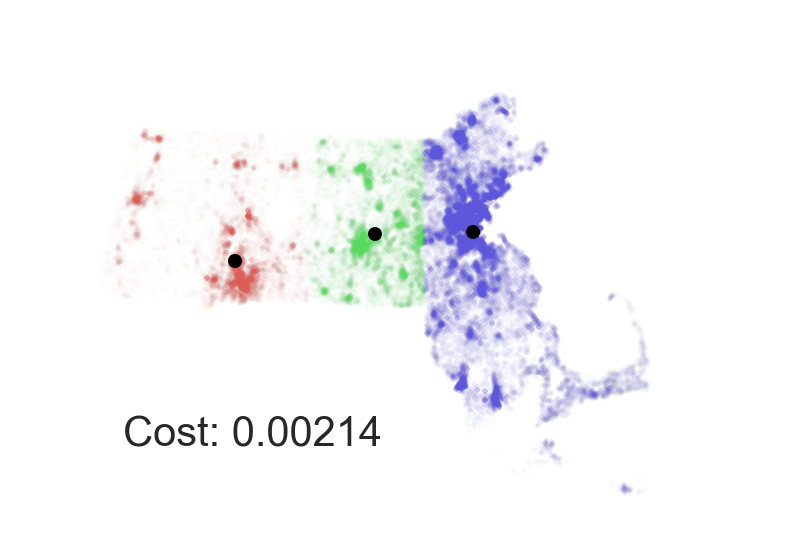
\includegraphics[width=5.5cm]{images/solution_sqrtwt_clusters3_minpop1.png} }}%
  \qquad
  \subfloat[$w(\xi)=\xi^2$]{{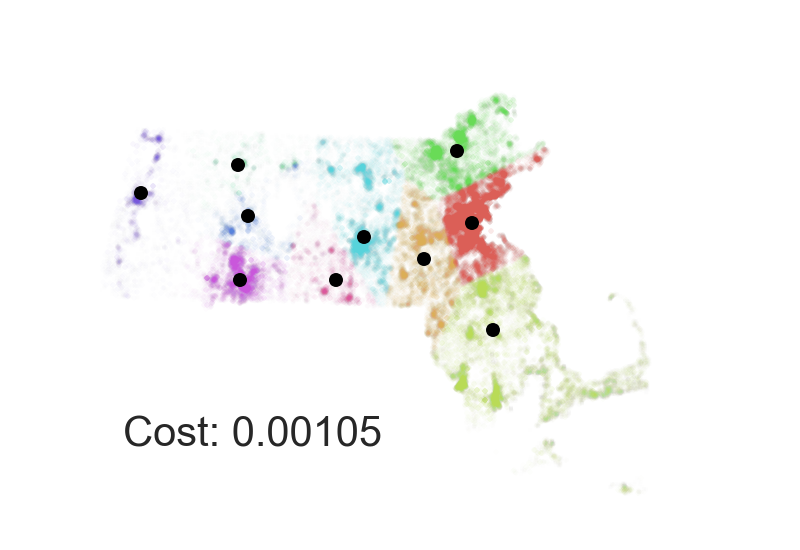
\includegraphics[width=5.5cm]{images/solution_sqwt_clusters10_minpop1.png} }}%
  \qquad
  \subfloat[$w(\xi)=\log(\xi)$]{{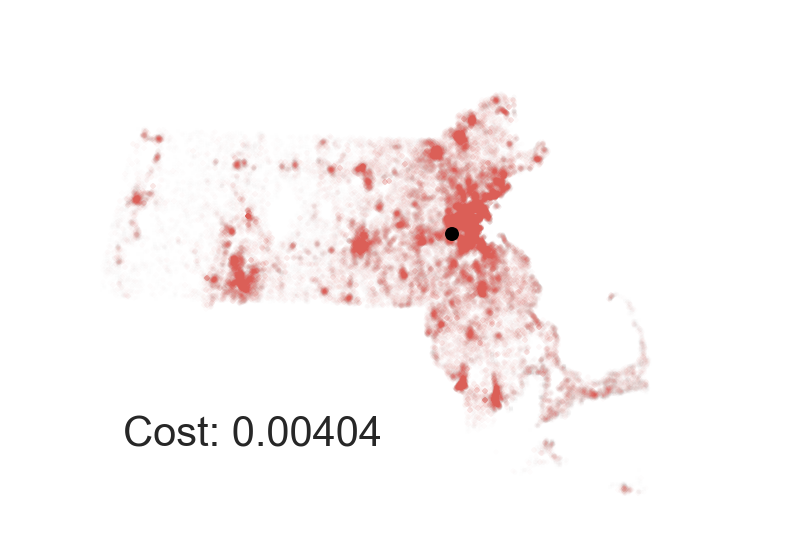
\includegraphics[width=5.5cm]{images/solution_logwt_clusters1_minpop1.png} }}%
%  \qquad
%  \subfloat[][$w(\alpha_i)=\begin{cases}\alpha_i, & \alpha_i > 1\\ 0, & \text{otherwise} \end{cases}$]{{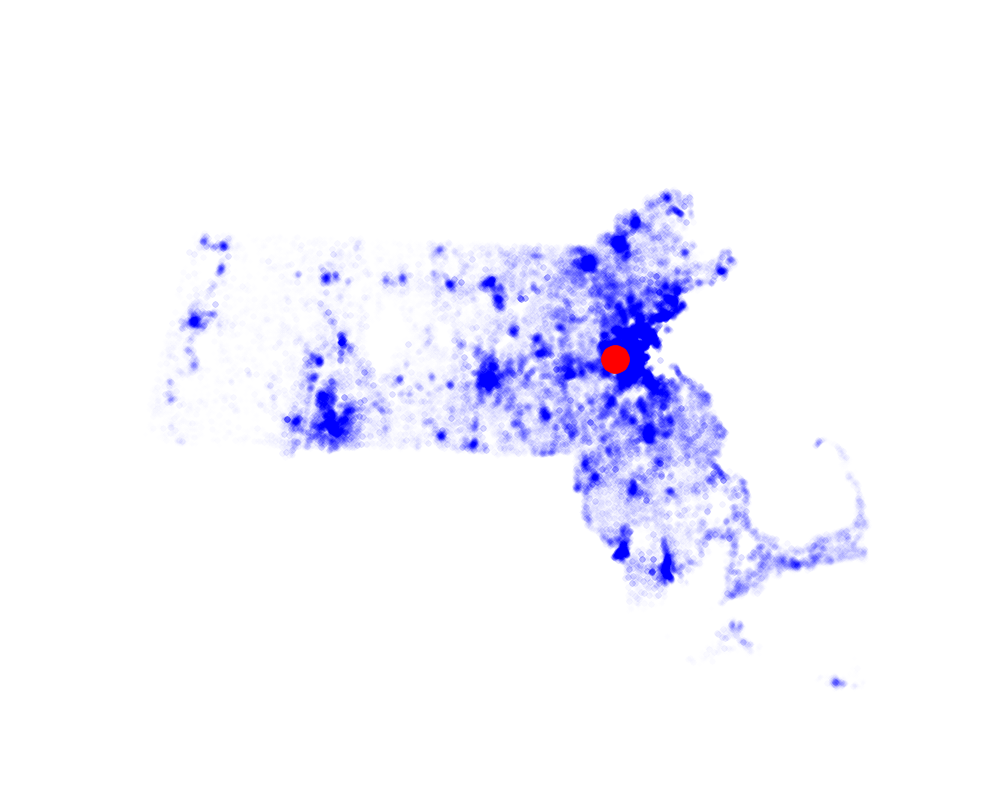
\includegraphics[width=5.5cm]{images/thresholdweight.png} }}
  \caption{Multiple distribution center placement under various weighting functions. The value of the cost function is displayed, and centers are shown in black.}
  \label{fig:centers}
\end{figure}

\section{Conclusions \& Future Work}
The choice of weighting function is a potential area of further, concentrated study. We assume that the weighting function is chosen based on \textit{a priori} domain knowledge, which suggests an investigation into data-driven choices of weighting functions for known business problems. The focus of this project was the development of an augmentation to Lloyd's algorithm that scaled with the number of clusters. We were successful to that end and are pleased with our clustering results.

Another interesting future variation that lends itself to study is how the clustering changes with the granularity of the population data. We utilized US Census\cite{census} block data that, while sufficiently detailed for a macro analysis of Massachusetts, is not detailed enough to provide adequate insight for the optimal location of distribution and/or retail centers within a densely populated city. If we had access to parcel data (storefronts and other properties at the street level) it is likely that our clustering solution would be fundamentally different from those presented in this paper.

\begin{thebibliography}{9}
  \bibitem{kmeans}
  Kanungo, T., Mount, D. M., Netanyahu, N. S., Piatko, C., Silverman, R., \& Wu, A. Y (2002). An Efficient $k$-Means Clustering Algorithm: Analysis and Implementation. \textit{IEEE Transactions on Pattern Analysis and Machine Intelligence 24}(7), pp. 881-892.
  \bibitem{lloyd}
  Lloyd, S. P (1982). Least Squares Quantization in PCM. \textit{IEEE Transactions on Information Theory 28}(2), pp. 129-137.
  \bibitem{census}
  U.S. Census Bureau. \textit{TIGER/Line� with Selected Demographic and Economic Data: Population \& Housing Unit Counts}. Retrieved from https://www.census.gov/geo/maps-data/data/tiger-data.html
  \bibitem{survey}
  Kolda, T. G., Lewis, R. M., \& Torczon, V (2003). Optimization by Direct Search: New Perspectives on Some Classical and Modern Methods. \textit{SIAM Review, 45}(3), pp. 385-482.
  \bibitem{charles}
  Davis, C. (1954). Theory of Positive Linear Dependence. \textit{Journal of American Mathematics, 76}(4), pp. 733-746.
  \bibitem{pyshp}
  \textit{Python Shapefile Library}. Github repository. Retrieved from https://github.com/GeospatialPython/pyshp
  \bibitem{1D}
  Chen, D. Z., Li, J., \& Wang, H. Efficient Algorithms for the One-Dimensional $k$-Center Problem (2015). \textit{Theoretical Computer Science 592}, pp. 135-142.
  \bibitem{blocks}
  Rossiter, K. (2011, July 20). What are census blocks? [Web log post]. Retrieved from http://blogs.census.gov/2011/07/20/what-are-census-blocks/
\end{thebibliography}
\end{document}